\providecommand{\rasd}{..}
\documentclass[../RASD.tex]{subfiles}

\begin{document}
    \chapter{Implementation, integration and test plan}\label{ch:implementation,-integration-and-test-plan}
    In this section there is the order in which we plan to implement the sub-components of our system
    and the order in which we plan to integrate such sub-components and test the integration.
    \section{Component implementation}\label{sec:component-implementation}
    The system development will only concern the UserMobileApp, since the server, the map and the storage will be provided by external companies.
    The system will be implemented, but also tested and integrated, following a bottom-up strategy.
    The external system’s components will not need to be implemented and tested, since they can be considered reliable.
    Nonetheless, the interaction with these systems will need to be tested as well, to check that it has been properly interfaced with SafeStreets.
    Since the features have different importance in the context of the application, the following table will resume some consideration on each functionality
    in the context of the application, the user and the development.
    In particular, the importance for the customer will consider the impact on the customer itself in his experience inside the application and the reasons
    that could bring him to join and use SafeStreets;
    the importance for SafeStreets will consider the possible impact of SafeStreets in the market, the use that it could do to improve the system itself
    and the possible legal aspects;
    the implementation difficulty will provide a qualitative estimation of the amount of work and time that will be needed to develop that particular feature.
    \newpage
    \begin{center}
        \begin{longtable}{| p{.25\linewidth} | p{.25\linewidth} | p{.25\linewidth} | p{.25\linewidth} |}

            \hline
            \textbf{Feature} & \textbf{Importance for the customer} & \textbf{Importance for SafeStreets} & \textbf{Implementation difficulty} \\ \hline
            Sign up and login & Low & Medium & Low\\ \hline
            Violation reporting & Very High & Very High & Medium\\ \hline
            Visualization of customer’s own reports & Medium & Low & Low\\ \hline
            Daily map visualization & High & High & High\\ \hline
            Query all the violations & High & Medium & High\\ \hline
            Violation Visualization & High & High & Low\\ \hline
            Show/hide sensitive information & High & High & High\\ \hline
            Give a feedback to a violation & Medium & High & High\\ \hline
            Build statistics on the violations & Low & Medium & Medium\\ \hline
            Mark dangerous area & High & Medium & High\\ \hline
            Provide suggestions about unsafe areas & Low, for the users High, for the municipality & Low & Medium\\ \hline
            Mark violations as fined & Medium & Medium & Low\\ \hline
            \caption[\textit{Features importance}]{\textit{Features importance}}
        \end{longtable}
    \end{center}
    It is important to mark again that the core functionality of SafeStreets will be the violation reporting,
    and since almost all the other functionalities are based on the reported violations it is important to develop it as first.
    According with the considerations done, the features will need to be implemented and unit tested with the following order:
    \begin{itemize}
        \item \textbf{Violation reporting}: as previously said, this is the core functionality of the application.
        To develop this feature, the NewReport Manager will need to be partially developed and tested.
        Moreover, the correct integration in the system of the server and database must be ensured, at least in the upload task.

        \item \textbf{Sing up and login}: even if this feature is not considered to have an high impact neither for the user nor for safe street,
        it is important to implement it as soon as possible to match reports with the people who upload them.
        At this point, the NewReport Manager must be partially implemented and tested even in the functionality that concern the user matching.

        \item \textbf{Violation visualization}: this is one of the most important features of the system, and so it needs to be developed as soon as possible.
        To ensure that it work correctly, the ViewReport Manager must be partially implemented and tested,
        and the correct integration with the database and the server must be ensured even for what concerns the download functionalities.

        \item \textbf{Query all the violations}: This is another core functionality of the system, and so must have a high priority in developing it.
        Even if the main part of this functionality is done by the database provider, it is important to implement and meticulously test the ViolationQuery Manager,
        since it is used by other managers.

        \item \textbf{Daily map visualization}: to provide this functionality, the ViolationMap Manager must be almost fully implemented and tested,
        and its integration with the ViolationQuery Manger (already implemented for the violation query feature) must be tested as well to ensure
        that they interact correctly.
        The integration with the map provider must also be checked to work correctly.

        \item \textbf{Visualization of customer’s own reports}: this is not a core functionality of the system;
        however, since it could be considered important for some of the users and most of its components should be already have been implemented at this point,
        it could be useful to add it to the application.
        The ViolationQuery Manager is the only component on which this feature is based, so the last feature functionality of this manager
        must be implemented if needed and eventually tested.

        \item \textbf{Show/hide sensitive information}: this is the most critical feature of the whole system, since if it does not work correctly
        the sensitive information will risk being shown to all the users.
        Because of that, the NewReport Manager must be fully implemented at this point, as well as the integration of the plate recognizer,
        and they must be accurately tested.

        \item \textbf{Give a feedback about a violation}: this feature is not crucial but is important to let the community limit the wrong reporting.
        To do that, the UserReportVisualization Manager must be implemented in all the functionalities that concern the feedback upload,
        and they must be tested as well.

        \item \textbf{Mark dangerous area}: this feature is one of the most difficult to implement but is at the same time one of the most useful for the users.
        An algorithm must be designed to identify the potential unsafe area, and the UnsafeArea Manager must be implemented in all the functionality
        that are used to define them.
        Because of the possible difficulties that could rise in the development phase, the testing of this feature must be very accurate.

        \item \textbf{Provide suggestions about unsafe area}: to provide this feature, the UnsafeAreaManager must be implemented with the last functionalities
        that are missing from the previous point.
        The algorithm to identify the possible interventions must be designed as well, and everything must be finally tested.

        \item \textbf{Mark reports as fined}: even if this is one of the easiest features to develop,
        it is less important than the others for both the users and SafeStreets, and so is one of the last to be developed.
        The UserReportVisualization Manager must implement the last functionality to enable this feature, and they must be tested as well.

        \item \textbf{Build statistics on the violations}: this is the last feature to be implemented, because it will use the data collected
        by all the other functionalities and would be less important without them.
        The Statistics Manager must be fully implemented and tested.
    \end{itemize}
    It is important that the testing run in parallel with the implementation of the system whenever is possible, in order to spot possible errors
    as soon as possible and avoid propagating them on the following features.
    Whenever the integration of two or more components have to be integrated,
    it is important that will be unit-tested first, to limit as much as possible the presence of errors and bugs.
    Once the system will be fully integrated, it will have to be tested again to test that all the functional and non-functional requirements hold.
    Moreover, since the system is thought to work with a big amount of data, some performance tests will have to be done.
    Even if most of them will be possible only once that the system is fully integrated, these tests must be introduced as soon as possible,
    to detect possible data structure or algorithm that may cause a bad computation of data.
    \newpage
    \subsection{Provider choice}\label{subsec:provider-choice}
    \begin{itemize}
        \item \textit{Requirements:}
        \begin{itemize}
             \item \textbf{Authentication provider}:\newline Regarding the authentication provider we want a service that can:
             \begin{enumerate}
                 \item Register new users
                 \item Authenticate the registered one
             \end{enumerate}
             The best effort is the encryption of the password that is useful in terms of security.
             \item \textbf{Map provider}: \newline It’s fundamental in SafeStreets app to display reports on a map.
             Furthermore, the map provider must be able to display the position of the user and the reports on the map.
             \item \textbf{Plate recognizer provider}: \newline In order to recognize a plate from a picture, we decided to choose a provider
             that it’s able from a photo to return a readable file with plate and pixels of it as strings (if present).
             \item \textbf{Database provider}: \newline Database systems are complex, difficult and time-consuming to design and for the developers require
             an initial training, so from this point of view is more convenient to take one ready-made.
             We want a database that stores reports with all their information and also be able to retrieve information about one user from his mail.
        \end{itemize}
        \item \textit{Implementation choice}: \newline To satisfy all these requirements we choose to lean on \textit{Firebase}
        for the authentication and database functionality. \textit{Firebase} is a Backend-as-a-Service (BaaS) app development platform that provides
        hosted backend services.
        One of them is \textit{Firebase Auth} that provides backend services to authenticate users to our app.
        It supports authentication using passwords, phone numbers, popular federated identity providers like Google, Facebook and Twitter, and more.
        Another services that comes from \textit{Firebase} is \textit{Cloud Firestone}.
        It is a flexible, scalable NoSQL cloud database to store and sync data for client- and server-side development.
        In \textit{Cloud Firestore}, SafeStreets can use queries to retrieve individual, specific documents or to retrieve all the documents
        in a collection that match our query parameters.
        In this way SafeStreets queries can include multiple, chained filters and combine filtering and sorting.
        They're also indexed by default, so query performance is proportional to the size of the result set, not of the data set.
        \textit{Firebase Storage} provides secure file uploads and downloads, regardless of network quality.
        The developer can use it to store images, audio, video, or other user-generated content.
        For the map provider we choose \textit{Google Maps API}.
        It provides detailed and accurate maps of all the world.
        It also allows to customize the map for instance by adding markers.
        For the plate recognizer service we choose \textit{Plate Recognizer}.
        It takes an image as input and produces an easy to use JSON response with the number plate value of the vehicle and the pixels's location of that plate.
    \end{itemize}
    \newpage
    \section{Component Integration}\label{sec:component-integration}
    Each component should be integrated with the others only after it’s almost totally completed and with a satisfying unit testing’s result in order
    to avoid and contain the impact of each possible error, fault and failure on the system.
    For the same aim, right after a component has been integrated with the system, the relative integration testing should be made.
    The diagrams in the next sections show which components will go through the process of integration for a further clarification.
    The arrows start from the component which “uses” the other one.
    \subsection{Integration of the Application logic component}\label{subsec:integration-of-the-application-logic-component}
    Managers will be integrated with User mobile app and this will be the complete logic application.
    \begin{figure}[H]
        \centering
        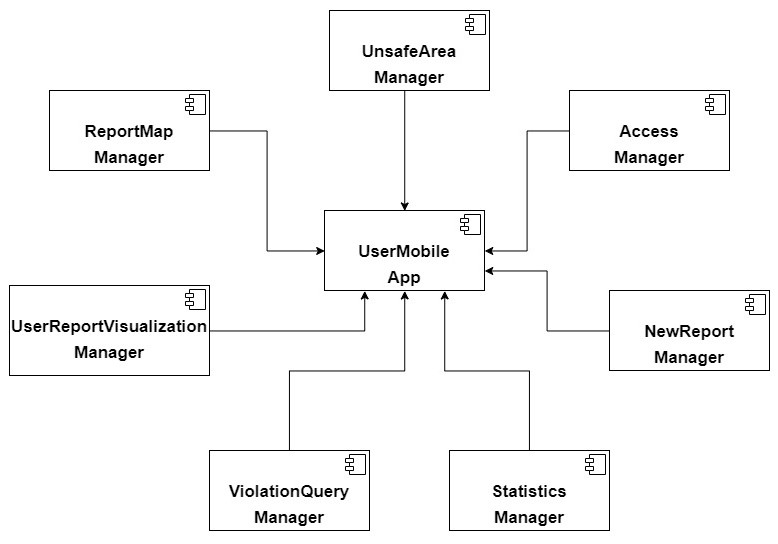
\includegraphics[scale = 0.8]{assets/integration_diagrams/user_mobile_app_integration.png}\\[1.6 cm]
        \caption[\textit{Integration} Diagram of the application logic]{Integration diagram of the application login.}
    \end{figure}
    \subsection{Integration of the internal component of the application logic}\label{subsec:integration-of-the-internal-component-of-the-application-logic}
    Components that use ViolationQuery functionalities are going to be completed only after they will be integrated with ViolationQuery manager.
    \\
    \begin{figure}[H]
        \centering
        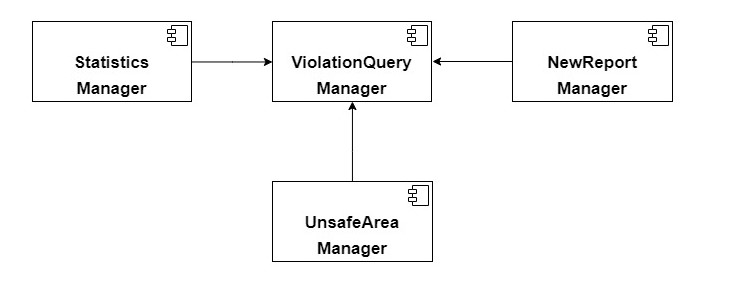
\includegraphics[scale = 0.8]{assets/integration_diagrams/violation_query_integration.png}\\
        \caption[\textit{Integration} Diagram of the internal component]{Integration diagram of the internal component.}
    \end{figure}
    \newpage
    \subsection{Integration of the external services}\label{subsec:integration-of-the-external-services}
    The integration of the external services is done only after each internal component is developed and tested sufficiently.
    \begin{figure}[H]
        \centering
        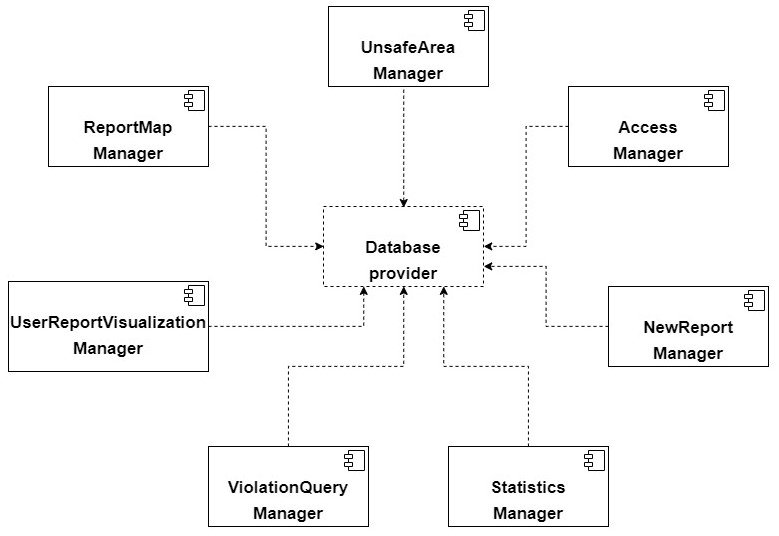
\includegraphics[scale = 0.8]{assets/integration_diagrams/database_provider_integration.png}\\[1.6 cm]
        \caption[\textit{Integration} Diagram of the database provider]{Integration diagram of the database provider.}
    \end{figure}

    \begin{figure}[H]
        \centering
        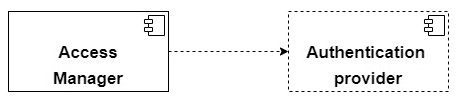
\includegraphics[scale = 0.8]{assets/integration_diagrams/authentication_provider_integration.png}\\[1.6 cm]
        \caption[\textit{Integration} Diagram of the authentication provider]{Integration diagram of the authentication provider.}
    \end{figure}

    \begin{figure}[H]
        \centering
        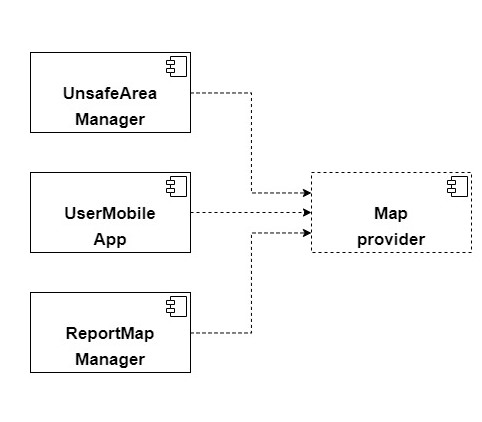
\includegraphics[scale = 0.8]{assets/integration_diagrams/map_provider_integration.png}\\
        \caption[\textit{Integration} Diagram of the map provider]{Integration diagram of the map provider.}
    \end{figure}

    \begin{figure}[H]
        \centering
        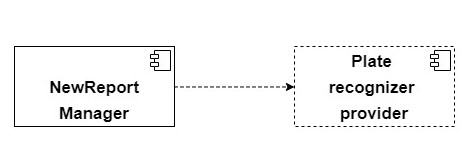
\includegraphics[scale = 0.8]{assets/integration_diagrams/plate_provider_integration.png}\\
        \caption[\textit{Integration} Diagram of the plate recognizer provider]{Integration diagram of the plate recognizer provider.}
    \end{figure}

    \begin{figure}[H]
        \centering
        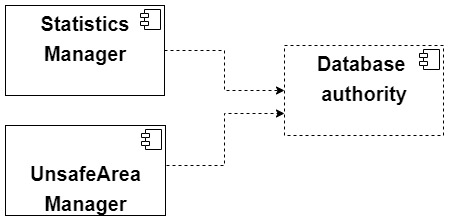
\includegraphics[scale = 0.6]{assets/integration_diagrams/db_authority_integration.png}\\
        \caption[\textit{Integration} Diagram of the authority database]{Integration diagram of the authority database.}
    \end{figure}

    \newpage
    \section{Algorithms}\label{sec:algorithm}
    This section will provide some general indication about the significant algorithms that will be developed within the system.
    \subsection{Unsafe Area Search}\label{subsec:unsafe-area-search}
    Determine the unsafe areas is one of the most critical aspect of the system, because of the lack of a objective criteria
    to determinate when an area is more dangerous than another.
    The data that will be used for this algorithm are the reports collected by SafeStreets and the accidents provided by the municipality.
    Each of them will be associated to some parameters that will be used to evaluate the impact that they have on the danger level of the area;
    for simplicity they will both be referred as reports from now on.
    \begin{itemize}
        \item \textbf{dangerLevel:} every report category will be associated with a value that will set the basic danger level of the area.
        \item \textbf{timePassed:} is a coefficient that will be decreased with the time passed from the reporting.
        The idea is that a report will be less relevant as the time from its occurrence passes.
        \item \textbf{influenceDistance:} is a parameter that sets the radius of the circle in which the report has a relevant influence.
        It can be different depending on the report category.
    \end{itemize}
    Since the accidents will be provided by the municipality, it will be possible that some information will miss: in that case, a default value will be assigned.
    The algorithm will work as following: every accidents will mark an unsafe area defined by its influenceDistance.
    To these areas will be assigned a value equal to their dangerLevel, eventually corrected with the timePassed parameter,
    and if some areas will overlap their danger level will be summed.
    Finally, the violations reported in the marked zone will be used to increment the unsafe level, according to their parameters.
    After processing the data, the system will check for the violations in the previously determined area that have a danger value
    beyond a certain threshold and will provide a default solution for the most reported category.



\end{document}
